%!TEX root = ClementiBarba2020.tex

\section{Rockstuhl replication}

These first set of results correspond to the replication study of some results 
of Rockstuhl et al, 2005 \cite{rockstuhl2005}. Rockstuhl and coworkers did a two dimension 
study of the phonon-polariton response of different nanoparticles of silicon carbide (SiC)
using a 2D boundary element method. Their limit their study to 2D shapes and assumed an infinite
third dimension. (They solved full maxwell in 2D)


We count with a 3D surface boundary element method solver, that uses the electrostatic approximation
($\lambda > d$ where $d$ is the characteristic length of the geometry). 

{\color{red}We initially produced the meshes with trimesh (not sure how to cite), later we stick to 
our own script}

Initially we attempted to perform a convergence study on the result of Figure 18a
of Rockstuhl and coworkers. This simulation consists on a "quadratic cylinder" (square)
of size $L=535$. We tried to perform convergence on a cube of the same size L, but
due to the due to the sharp edges of the geometry we were not able to see proper convergence. 
However, we did a grid independence study. We were able to show that going from a mesh of 15552 
triangles (density = 1.11x10$^-4$ $N/\text{\AA}$) to 19200 (density = 9.05x10$^-5$ $N/\text{\AA}$) 
triangles the simulations did not change at all (see Figure \ref{fig:cube535}).  

\begin{figure}
    \centering
    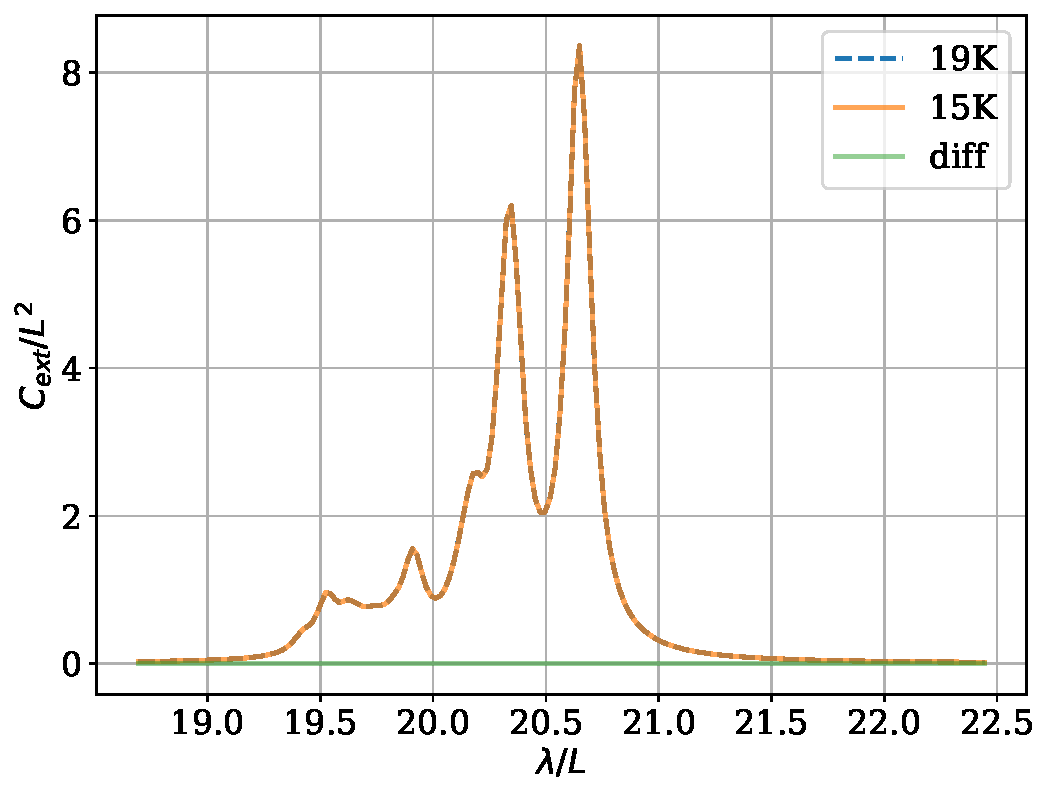
\includegraphics[width=0.85\textwidth]{cubeL535nm_15Kvs19K.pdf} 
    \caption{Extinction cross section divided by $L^2$ as a function fo wavelength divided by $L$ of
    a cube of size L=535 nm}
    \label{fig:cube535}
 \end{figure}

In this results we see extra peaks that we believe is due to the nature of our 3D model, in this case 
we have not extended the third dimension to approximate "infinity", but we suspect the extra peaks are 
due to sharpness of the edges (they mention this on their paper too) as well as the 3D nature of our solver.

These figure doesn't have the results digitized from the paper, but if needed we can add them. 

Based on these results we used the density of the cube as a reference to produce the meshes for the replication 
of figures 14a and 14b on Rockstuhl's work (case a1=672, b=328). This simulation is a "rectangular cylinder" of 
dimensions (we chose a case that will go well with our quasistatic model) are $a=672$ nm and $b=328$ nm. 

Effect of extended third dimension (in our case this is the y axis) are in Figures \ref{fig:ext_y_14a} and
\ref{fig:ext_y_14b}

\begin{figure}
    \centering
    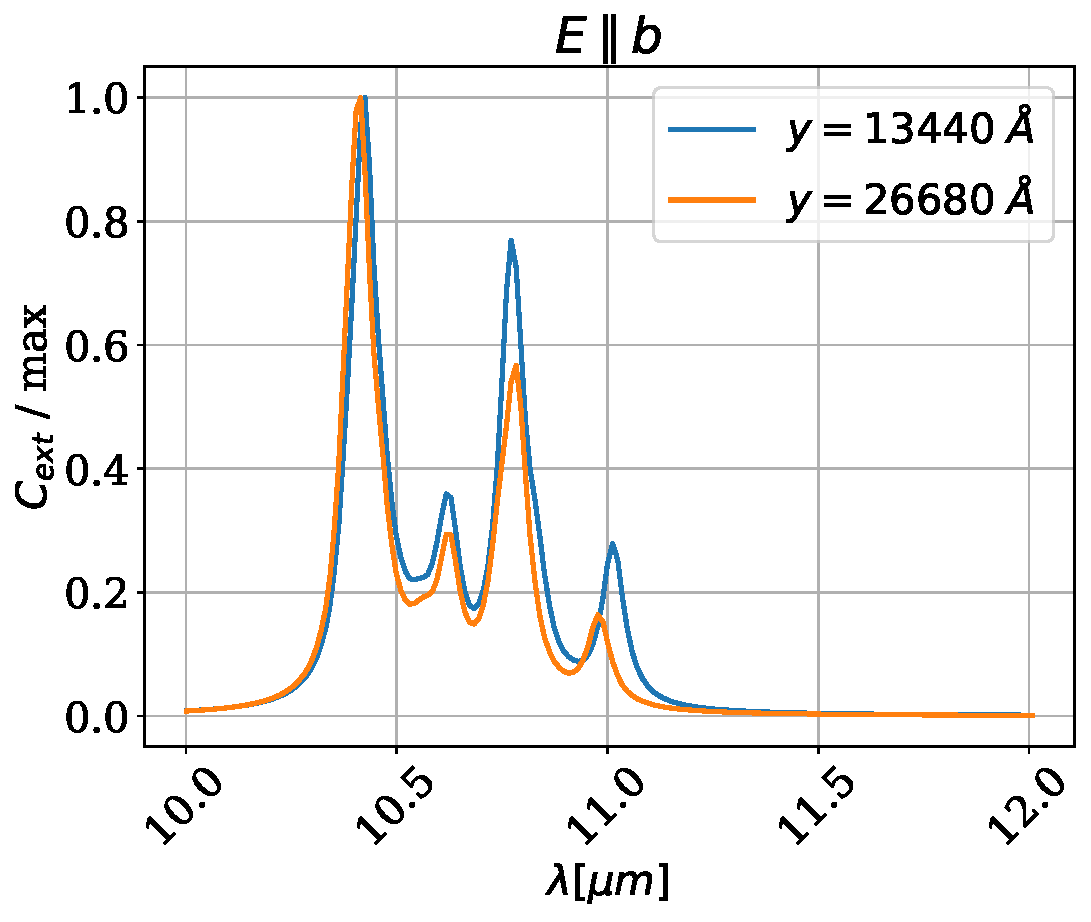
\includegraphics[width=0.85\textwidth]{ext_y_14a.pdf} 
    \caption{Normalized (by max) Extinction cross section of a rectangle for two different y-values in the 
    short edge configuration (electric field parallel to the shorter dimension)}
    \label{fig:ext_y_14a}
 \end{figure}

 \begin{figure}
    \centering
    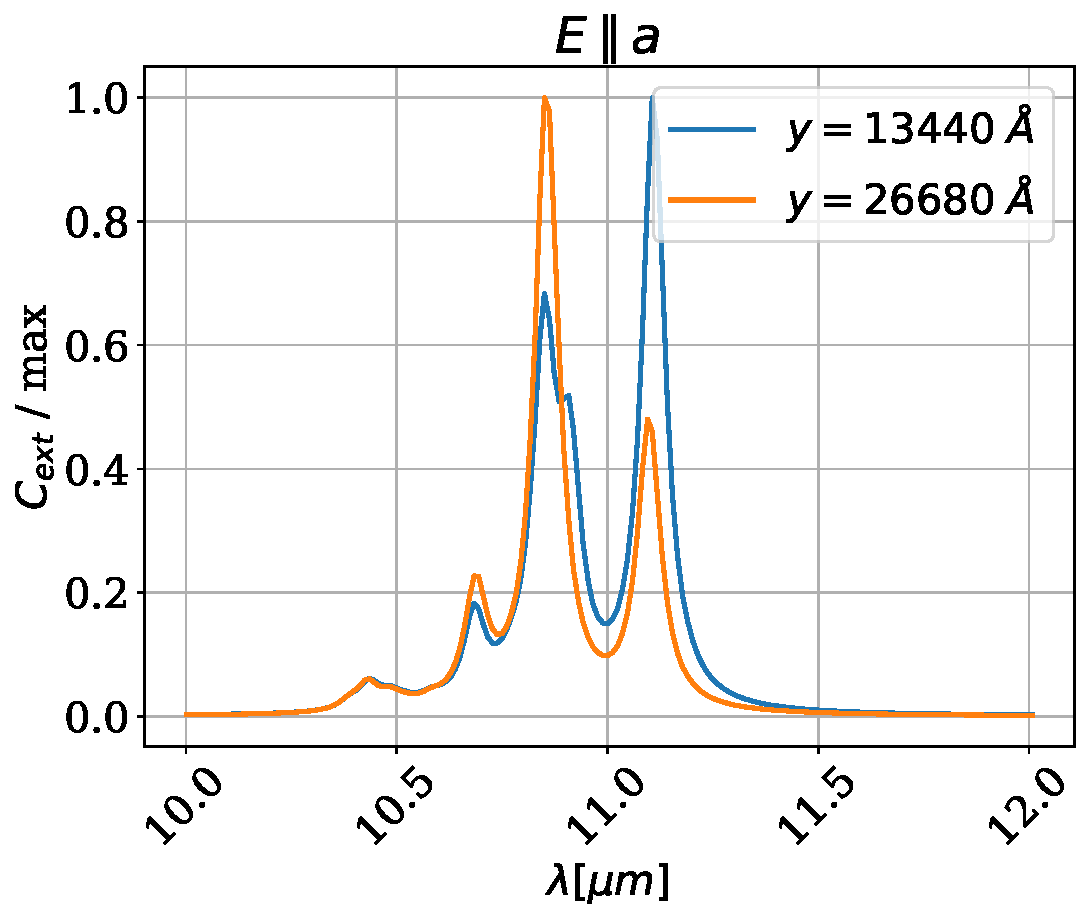
\includegraphics[width=0.85\textwidth]{ext_y_14b.pdf} 
    \caption{Normalized (by max) Extinction cross section of a rectangle for two different y-values in the 
    long edge configuration (electric field parallel to the longer dimension)}
    \label{fig:ext_y_14b}
 \end{figure}

We see that as we elongate the third dimension the extra peaks start fading. 

At this point we noticed that the mesher (trimesh) was not generating a uniform mesh. We created our 
own mesher, and tested the difference. Moreover, the paper mentioned that they rounded the corners of their
"rectangular cylinder". We were able to give our mesh as input to trimesh and round the edges but we were not able 
to know how the roundness was related to the arc of the curvature. This were parameters with no physical meaning, 
therefore we decided to go with the default setting. 


\begin{figure}
    \centering
    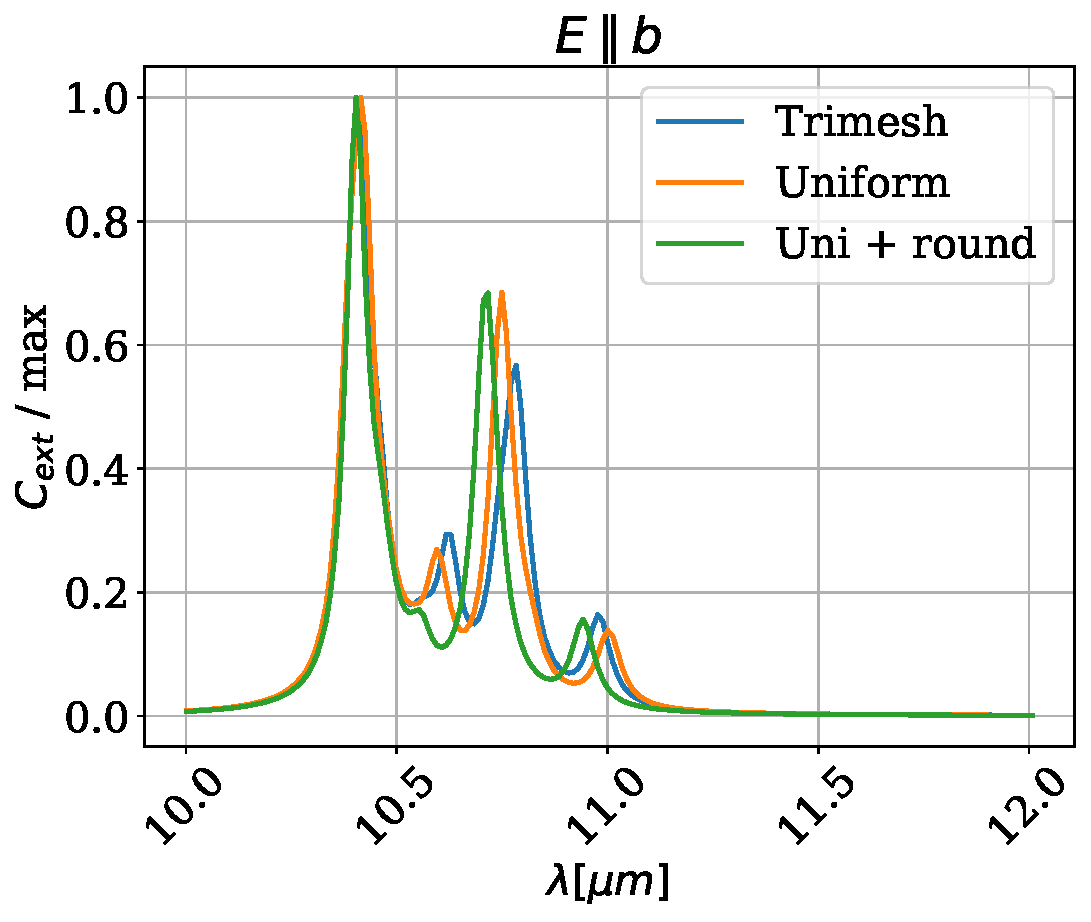
\includegraphics[width=0.85\textwidth]{tri_reg_round_14a.pdf} 
    \caption{Normalized (by max) Extinction cross section of a rectangle. Original trimesh, regular, and regular with 
    roundness. Short edge configuration (electric field parallel to the shorter dimension)}
    \label{fig:tri_reg_round_14a}
 \end{figure}

 \begin{figure}
    \centering
    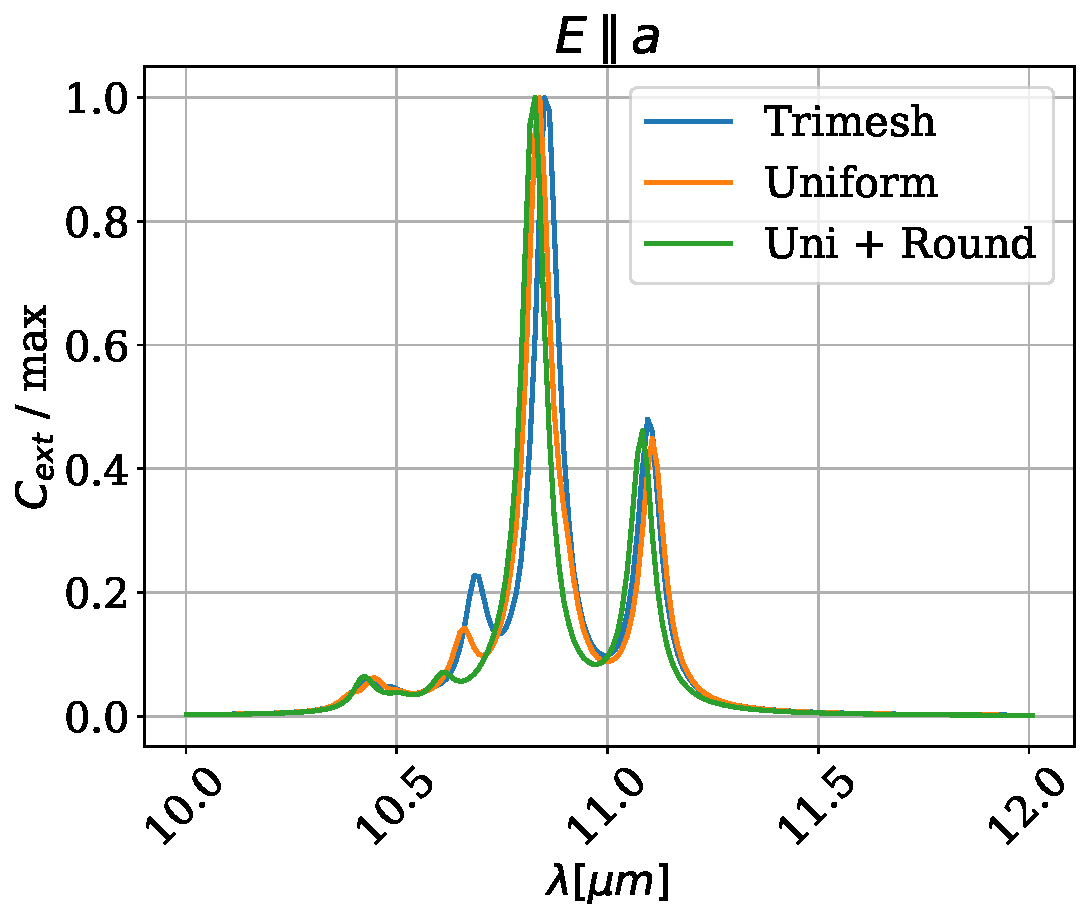
\includegraphics[width=0.85\textwidth]{tri_reg_round_14b.pdf} 
    \caption{Normalized (by max) Extinction cross section of a rectangle.  Original trimesh, regular, and regular with 
    roundness. Long edge configuration (electric field parallel to the longer dimension)}
    \label{fig:tri_reg_round_14b}
 \end{figure}


 Finally with all this info, here is the replication of Figures 14a and 14b. 

 \begin{figure}
    \centering
    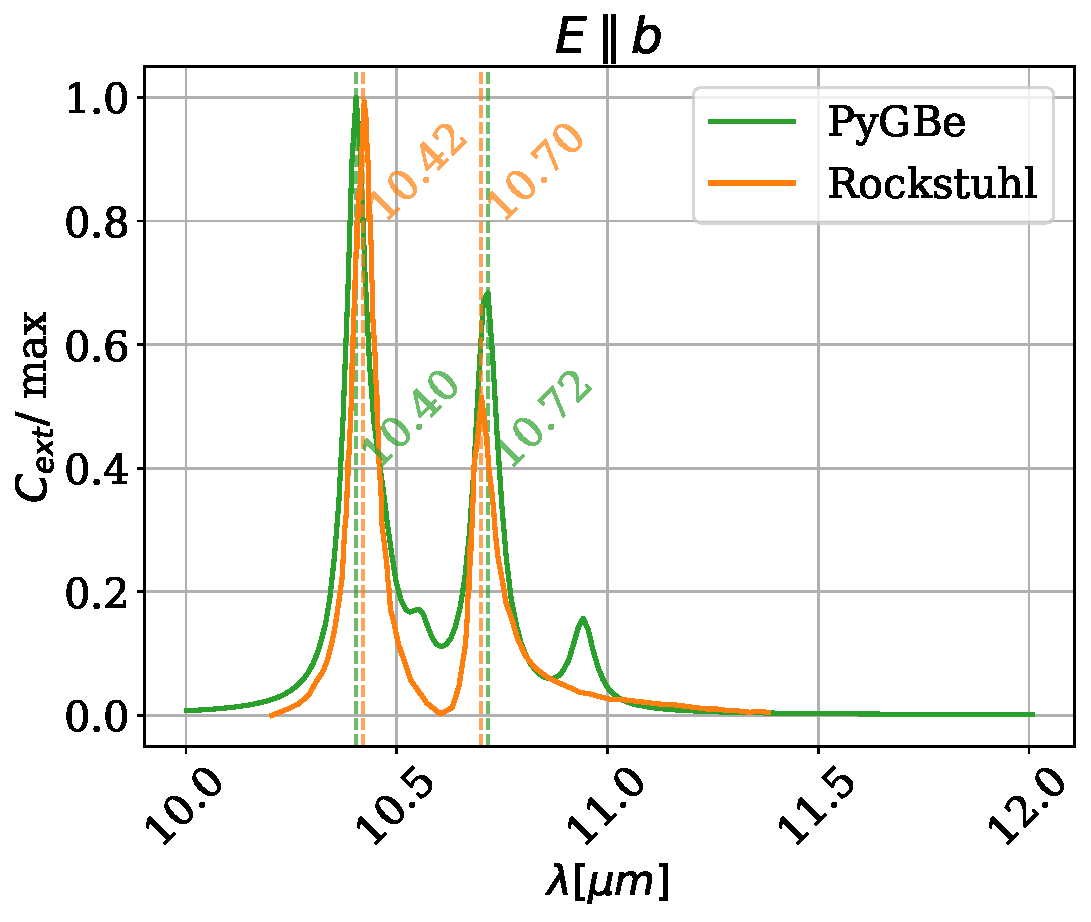
\includegraphics[width=0.85\textwidth]{replication_14a.pdf} 
    \caption{Normalized (by max) Extinction cross section of a rectangle. Replication of 
    the short edge configuration (electric field parallel to the shorter dimension)}
    \label{fig:rep_14a}
 \end{figure}

 \begin{figure}
    \centering
    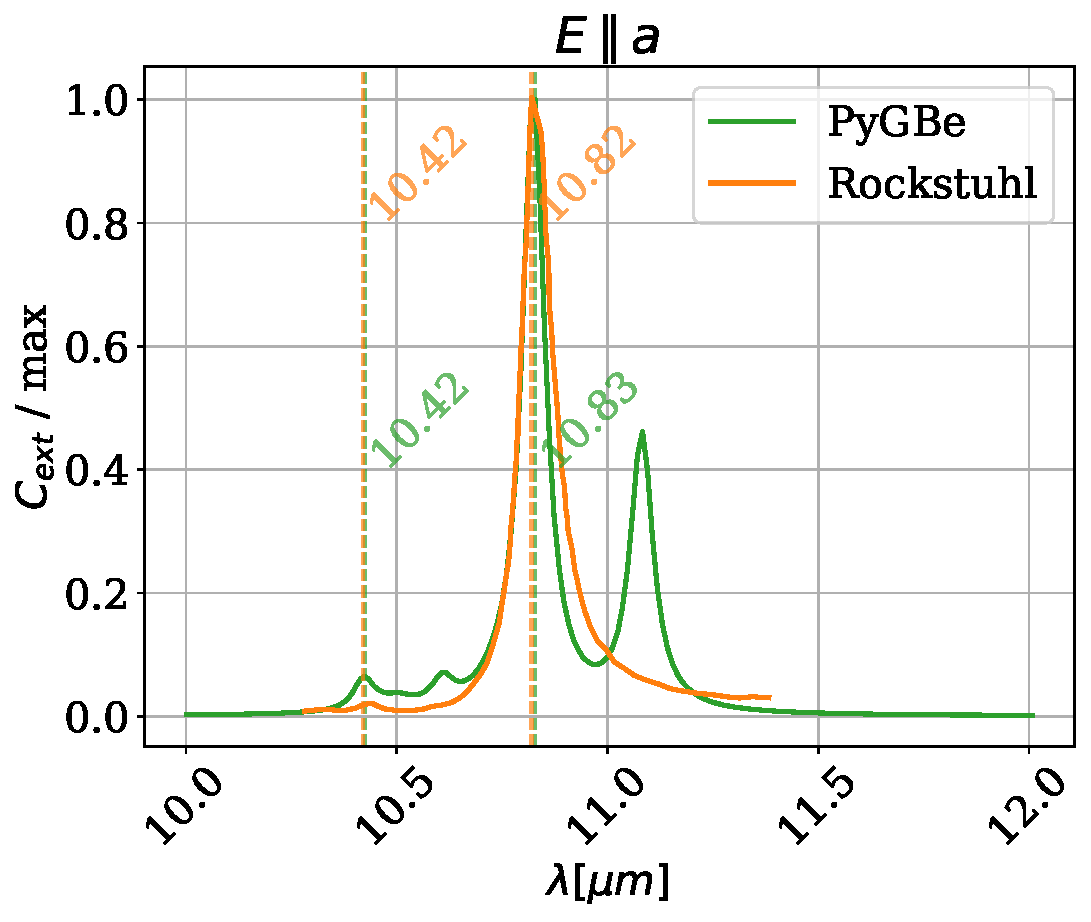
\includegraphics[width=0.85\textwidth]{replication_14b.pdf} 
    \caption{Normalized (by max) Extinction cross section of a rectangle. Replication of the 
    long edge configuration (electric field parallel to the longer dimension)}
    \label{fig:rep_14b}
 \end{figure}

 \section{Ellis replication and validation}

There are two results from this paper that we aim to replicate, and one of them is a comparison
against experimental results which will lead to a validation. 

The first result we show is a replication of a result presented in their supplementary 
material FigureS4 {\color{red}(note sure how to cite this, maybe a link)}. We aimed to replicate the 
black curve since the simulation setup is possible to replicate using PyGBe. For each aspect ratio (AR) 
value from 1 to 7 we computed the extinction cross section $C_{ext}$ across the wave number in the range
800-1000 $cm^{-1}$, we identify the the lower frequency mode ($E_{100}$ in Ellis paper)  that is not a 
longitudinal mode. We identify the Longitudinal modes by comparing normal vs 22 deg incidence runs. These
modes due to its nature do not show up in the normal incidence runs. Then, on the 22 deg incidence 
computations we choose the lower wave number mode that it's not a longitudinal mode. The simulations were 
performed for the Long Edge orientation, meaning that the electric field is polarized along the long edge 
of the pillar that is not the height. 

\begin{figure}
    \centering
    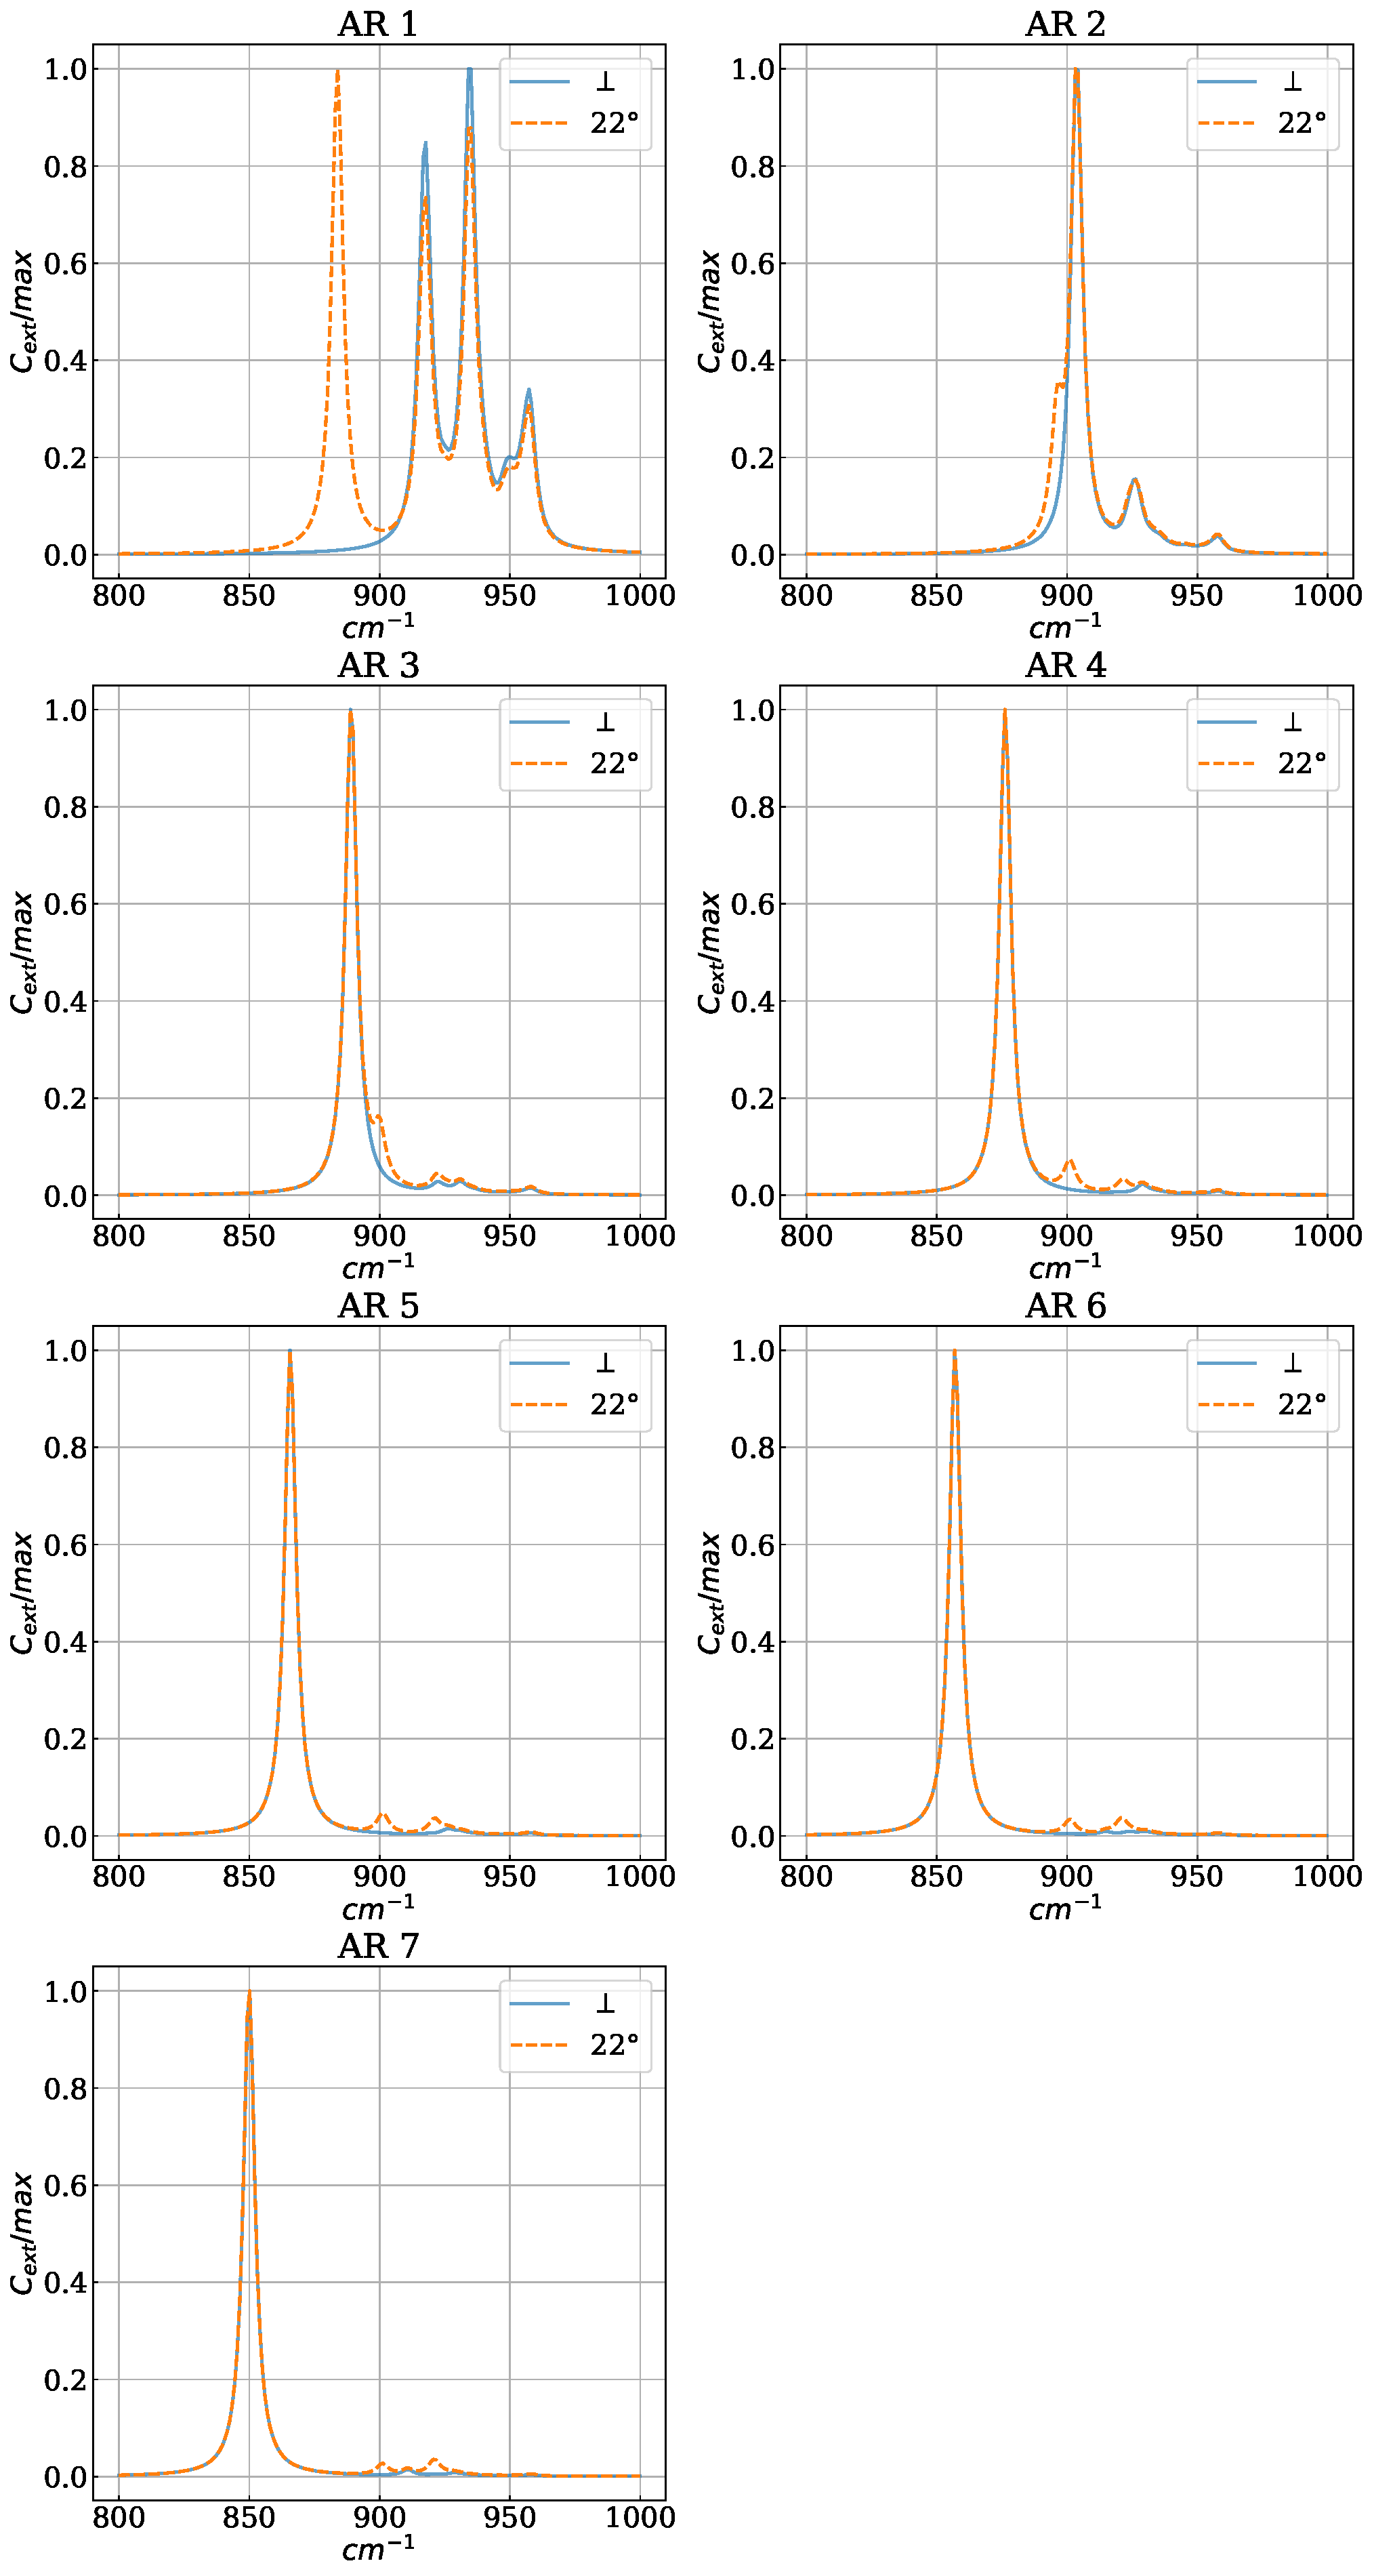
\includegraphics[width=0.95\textwidth]{AR_22_vs_norm.pdf} 
    \caption{ Extinction cross section across wave number for SiC pillars of multiple Aspect ratios. 
             (H=950 nm, W=400nm, L=400-2800 (AR=1-7))
            Normalized by maximum extinction cross section as a function of wave number,
            for a pillar orientation such that the electric field is parallel polarized 
            (I HAVE TO EXPLAIN THIS BETTER, IT ALIGNS WITH THE LENGTH OF THE PILLAR). 
            We present the results for normal incidence and 22 degrees incidence, 
            for different aspect ratios (AR)
            }
    \label{fig:AR_22_vs_norm}
 \end{figure}

THIS ARE THE PEAKS OF FIGURE \ref{fig:AR_22_vs_norm} need to find a better way of 
present these numbers. 

AR 1 peaks at frequency\\
normal: [ {\color{green}917.73} 934.092 949.604 957.325]\\
22 deg: [ {\color{red}883.926} {\color{green}917.73} 935.052 949.604 957.325]\\

AR 2 peaks at frequency\\
normal: [ {\color{green}903.233} 926.395 944.762 958.242]\\
22 deg: [ {\color{red}896.517} {\color{green}903.233} 926.395 944.762 958.242]\\

AR 3 peaks at frequency\\
normal: [ {\color{green}888.793} 922.552 931.223 948.613 958.242]\\
22 deg: [ {\color{green}888.793} 899.418 922.552 931.223 958.242]\\

AR 4 peaks at frequency\\
normal: [ {\color{green}876.186} 929.32 946.639 958.242]\\
22 deg: [ {\color{green}876.186} 901.281 921.618 929.32 945.745 958.242]\\

AR 5 peaks at frequency\\
normal: [ {\color{green}865.576} 926.395 945.745 958.242]\\
22 deg: [ {\color{green}865.576} 901.281 921.618 958.242]\\

AR 6 peaks at frequency\\
normal: [ {\color{green}856.904} 914.793 923.489 929.32 946.639 958.242]\\
22 deg: [ {\color{green}856.904} 901.281 920.6 958.242]\\

AR 7 peaks at frequency
normal: [ {\color{green}850.134} 910.963 921.618 928.372 946.639 958.242]
22 deg: [ {\color{green}850.134} 901.281 910.963 920.6 958.242]

In other words, we choose the lower mode (lower wavenumber) from the normal 
incidence cases.

Our simulations differ on the method and we do not have a substrate included. The black curve on 
Ellis et al \cite{ellis2016} represents the resonance positions for the $E_{100}$ mode for the different 
aspect ratios when the pillar are separated by a 5000 nm gap. The simulations performed with \pygbe 
consist of one isolated pillar.

\begin{figure}
    \centering
    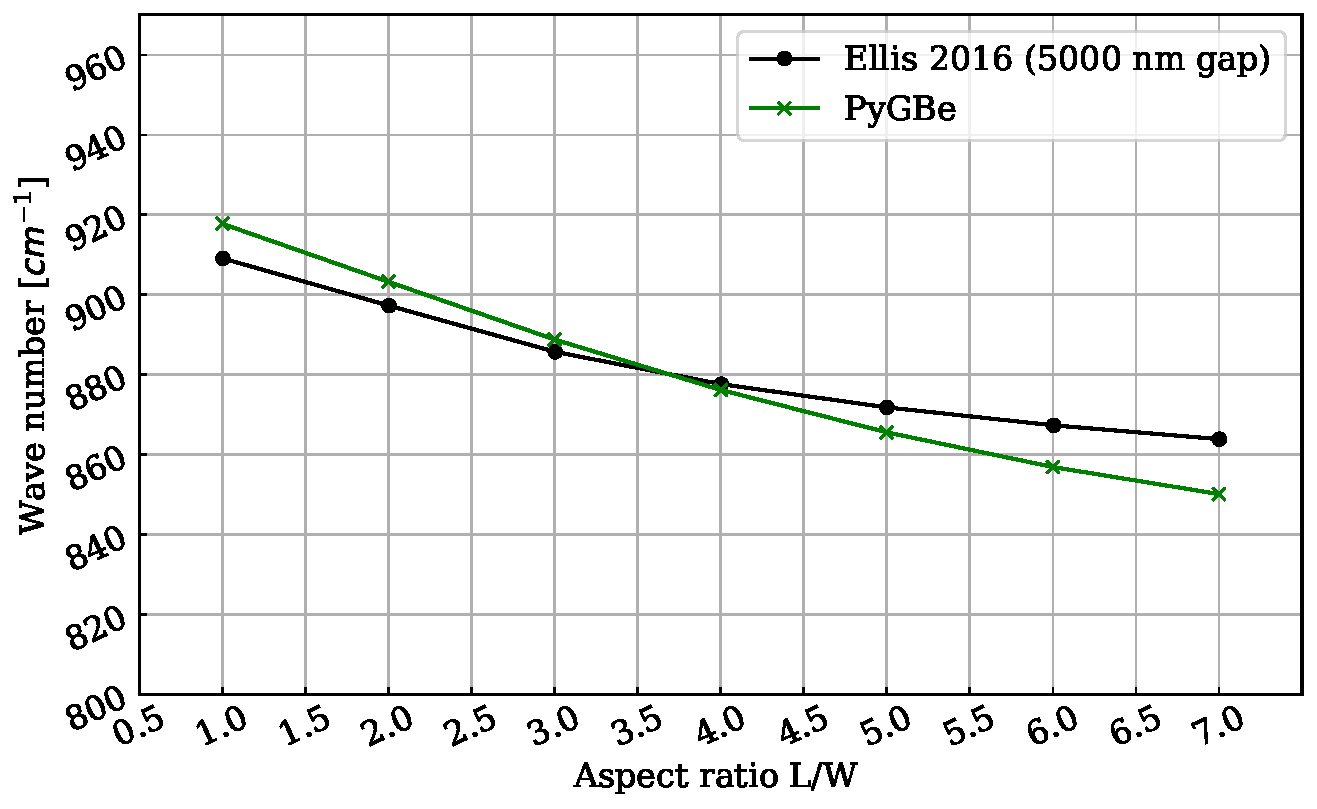
\includegraphics[width=0.85\textwidth]{AR_rep_FS4_Ellis2016.pdf} 
    \caption{Replication of figure S4 of supplementary material of Ellis 2016}
    \label{fig:rep_FS4_ellis}
 \end{figure}

 If we calculate de relative percentage error for each of these points we get:
 
 \begin{table}
    \centering
    \caption{\label{table:err_AR} Percentage error for different aspect ratios.} 
    \begin{tabular}{c c}
    \hline%\toprule
    ARR & \% error \\
    \hline%\midrule
     $1$ & $0.95$ \\
     $2$ & $0.67$ \\
     $3$ & $0.35$ \\
     $4$ & $0.16$ \\
     $5$ & $0.72$ \\
     $6$ & $1.20$ \\
     $7$ & $1.59$ \\
    \hline%\bottomrule
    \end{tabular}
\end{table}


\pygbe AR=4 attempt of validation Figure 2a (see Figure \ref{fig:pygbe_vs_exp_2a})

\begin{figure}
    \centering
    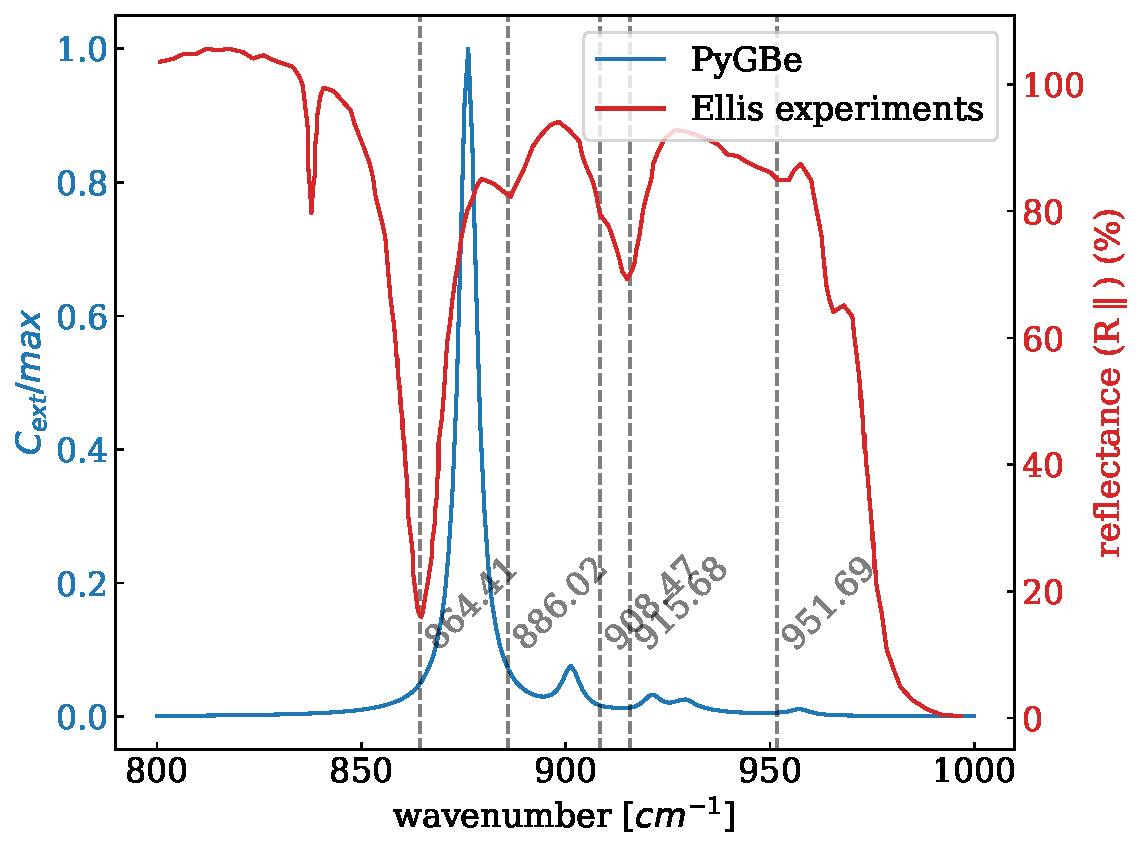
\includegraphics[width=0.85\textwidth]{pygbe_vs_exp_fig2a_Ellis.pdf} 
    \caption{\pygbe vs experiments, figure 2a of Ellis 2016. Ellis et al 
    has near field interaction in its experiments. Ellis data was digitized
    with web digitizer.}
    \label{fig:pygbe_vs_exp_2a}
 \end{figure}

First order approximation to achieve validation. In our code we do not have near 
field interaction. From Figure S4 in supplementary material of Ellis et al. We know that 
for the first mode ($E_{100}$) the difference between interaction and no interaction is 
12.17 $cm^{-1}$ (obtained from digitized data). If we use this as a first order approximation,
we can subtract that value from our curve, and the results are in Figure \ref{fig:val_2a}

\begin{figure}
    \centering
    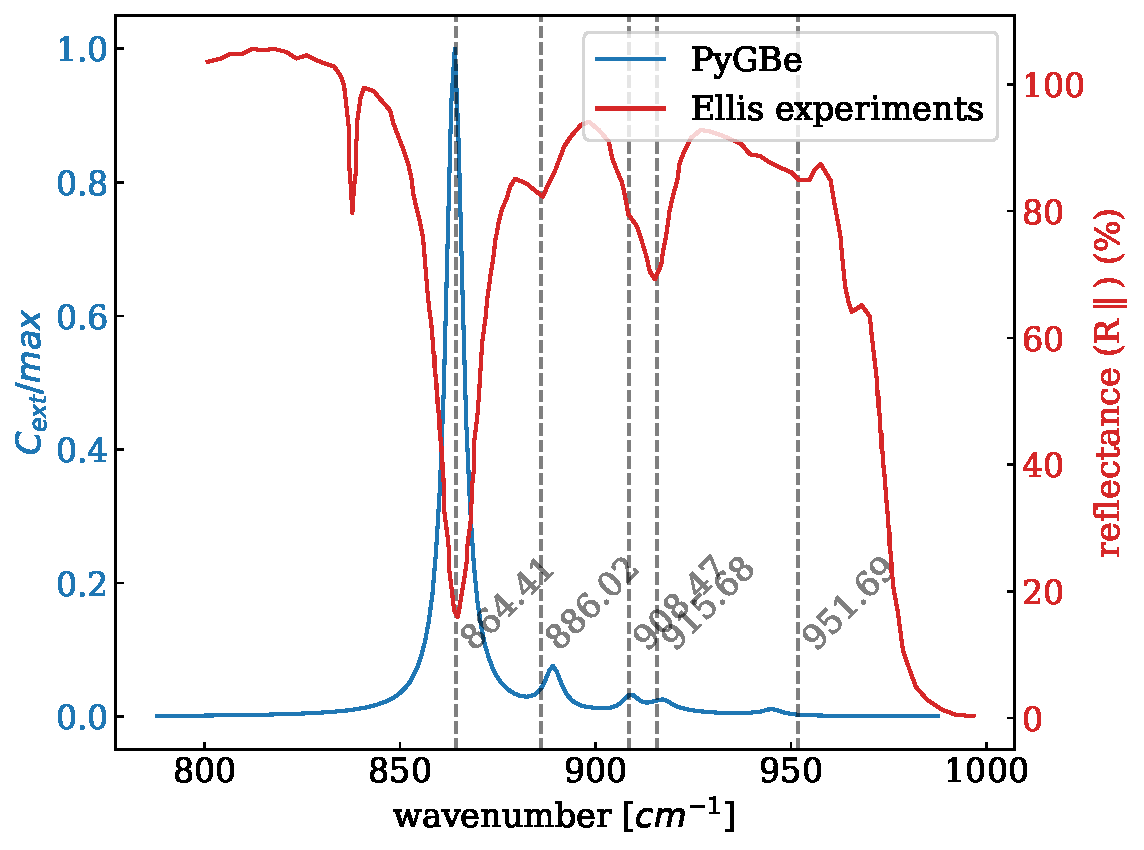
\includegraphics[width=0.85\textwidth]{validation_FOA_fig2a_Ellis.pdf} 
    \caption{Validation against experiments in figure 2a of Ellis 2016, using first order approximation}
    \label{fig:val_2a}
 \end{figure}

If we use the same approximation and compare the results with Ellis simulations on
Figure 2 of their paper (green curve) we get (see Figure \ref{fig:rep_2a})

\begin{figure}
    \centering
    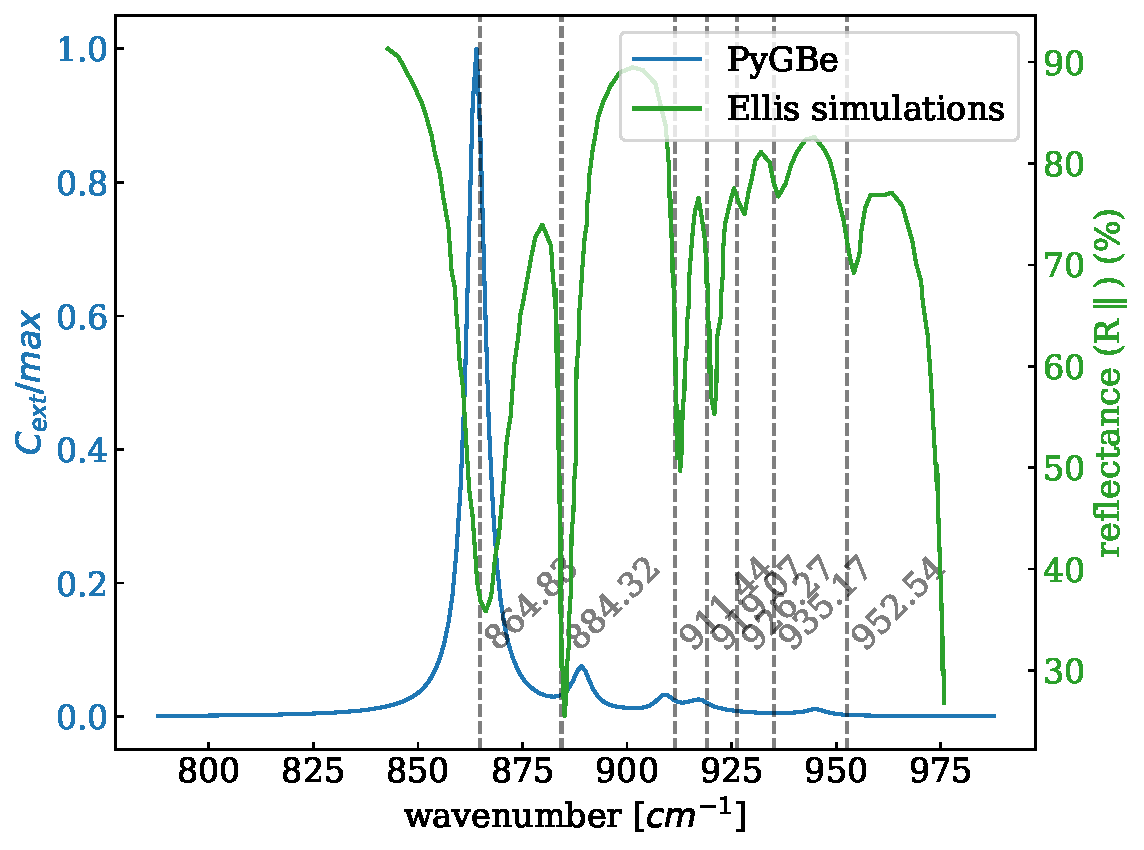
\includegraphics[width=0.85\textwidth]{replication_FOA_fig2a_Ellis.pdf} 
    \caption{Replication of simulations in figure 2a of Ellis 2016, using first
     order approximation}
    \label{fig:rep_2a}
 \end{figure}